\subsection{Double Slit Interference}

Illuminate two \textbf{closely spaced parallel slits}, the two slits acts as \textbf{coherent sources of waves}.
\begin{itemize}
    \item They emit light waves with a \textbf{constant phase difference} and the \textbf{same frequency}.
    \item E.g. use a bulb to illuminate a \textbf{narrow single slit}, then double slit arrangement is illuminated by light from the narrow single slit.
    \item Or just use a low power laser beam.
\end{itemize}

\textbf{Young's fringes} - alternate bright and dark fringes can be seen on a white screen where the diffracted light from the double slits \textbf{overlaps}. They are \textbf{evenly spaced} and \textbf{parallel to the double slits}.

The fringes are formed due to the \textbf{Interference of light} from the two slits
\begin{itemize}
    \item Where a \textbf{bright fringe} is formed, light from one slit \textbf{reinforces the light from the other slit}.
        \begin{itemize}
            \item The light waves from each slit \textbf{arrive in phase} with each other.
        \end{itemize}
    \item Where a \textbf{dark fringe} is formed, light from one slit \textbf{cancels the light from the other slit}.
        \begin{itemize}
            \item The light waves from each slit \textbf{arrive 180$^\circ$ out of phase}.
        \end{itemize}
\end{itemize}

\textbf{Fringes separation} is the distance between the centre of a bright fringe to the next bright fringe.
$$\text{fringe separation}\ w=\frac{\lambda D}{s}$$
where $s$ is the \textbf{slit spacing} and $D$ the distance from the silts to the screen.

The fringe becomes more widely spaced if
\begin{itemize}
    \item Distance $D$ from the slits to the screen is increased.
    \item Wavelength $\lambda$ of the light used is increased.
    \item The slit spacing $s$ is reduced.
\end{itemize}
The slit spacing is the distance between the \underline{centre of the slits}.

\subsubsection*{Theory of the Double Slit Equation}

\begin{center}
    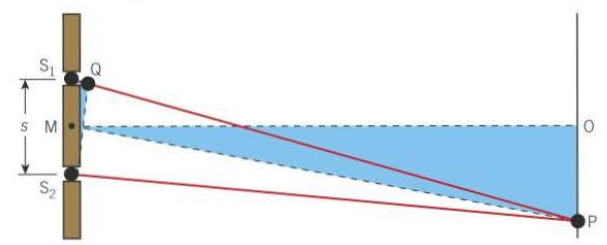
\includegraphics[width=5cm]{img/slits}
\end{center}

\begin{itemize}
    \item For \textbf{reinforcement} at $P$, the path difference $S_1P-S_2P=m\lambda$.
    \item For \textbf{cancellation} at $P$, the path difference $S_1P-S_2P=\left(m+\frac{1}{2}\right)\lambda$.
\end{itemize}
where $m=0,1,2$

Consider similar triangles
\begin{align*}
    \frac{S_1Q}{S_1S_2}&=\frac{OP}{OM}\\
    \frac{m\lambda}{s}&=\frac{mw}{D}\\
    w&=\frac{\lambda D}{s}
\end{align*}
The formula is only valid if the fringe separation $w$ is \textbf{much less than the distance} $D$ from the slits to the screen.
